\pagebreak
\subsection{Thermal Design} 
\label{Thermal_section}



\subsubsection{Optothermal considerations}

In order to ensure minimal measurement error in acquiring images, the effect of temperature on the optics must be considered, and the temperature must be controlled if needed to ensure that the error is within an acceptable range.\

\paragraph{SNR}

Dark current is small residual currents that are present in the camera, generated irrespective of whether there is incident illumination. This dark current becomes present in the data in the form of random noise that is not trivial to subtract. By decreasing the operating temperature of the camera optics, the magnitude of dark current can be minimised and the signal to noise ratio increased. This relationship between signal to noise ratio and dark current is as follows\\

\begin{center}
 $SNR =  \frac{I\times QE\times t}{\sqrt{I\times QE\times t+Nd\times t+Nr^2}}$\\
\end{center}

$I$ = Photon flux (photons/pixel/s)\\
$QE$ = Quantum efficiency\\
$t$ = Integration time (s)\\
$Nd$ = Dark current (electrons/pixel/s)\\
$Nr$ = Read noise (electrons)\\

The ASI183 camera is specified as having a read noise of 1.6e @30db gain and a QE peak of 84\%. The camera also has the following relationship between dark current and sensor temperature. Calculations will be considered for an exposure time of 300s, which is the longer intended exposure time for higher quality imaging.  \\


	\begin{figure}[h!]
    \centering
    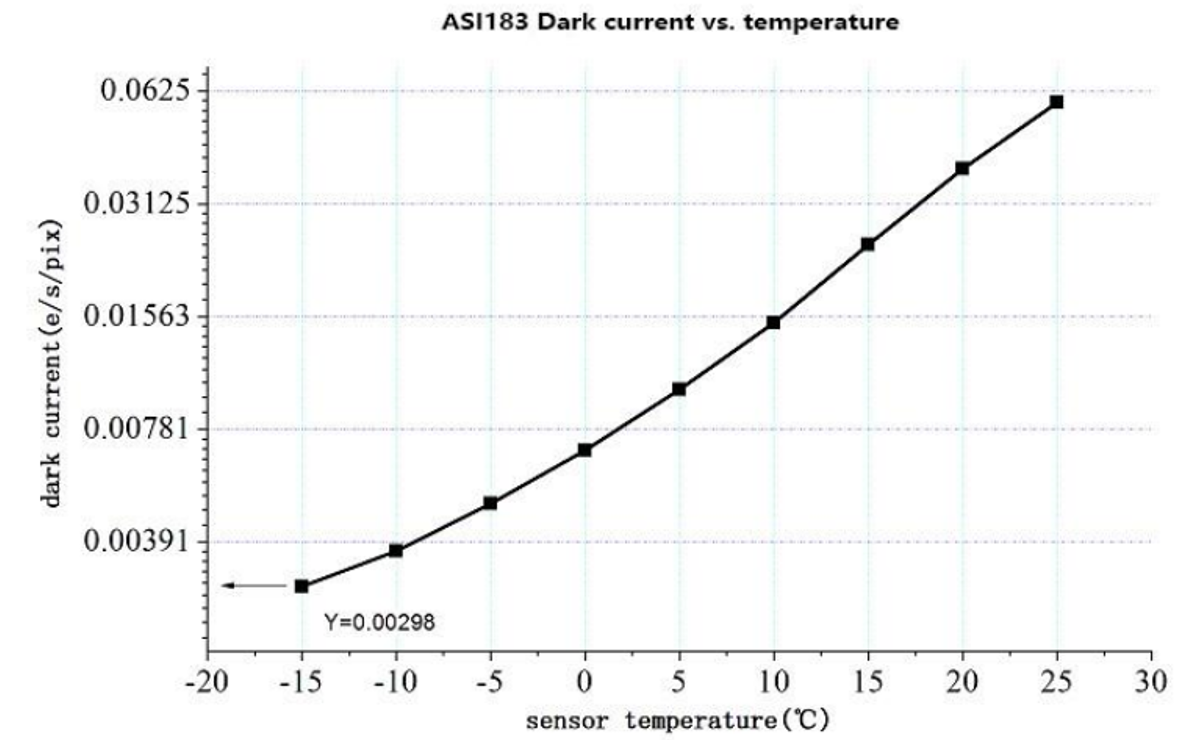
\includegraphics[scale=0.8]{4-experiment-design/img/mechanical/darkcurrent.png}
    	\caption{Dark current through the camera at various temperatures. Source: ZWO}
	\label{fig:darkcurrent}
	\end{figure}

As an example, the SNR as affected by dark current at -10\,\textsuperscript{o}C versus 10\,\textsuperscript{o}C is\\

 SNR(-10\,\textsuperscript{o}C) =  $\frac{(\SI{6.16}{photons \per pixel \per sec})\times (0.84)\times (\SI{300}{s})}{\sqrt{(\SI{6.16}{photons \per pixel \per s})\times (0.84)\times (300s)+(\SI{0.00391}{e \per pixel \per s})\times (\SI{300}{s})+(\SI{1.6}{e})^2}}$ \\

 SNR(-10\,\textsuperscript{o}C) = 39.35\\

 SNR(10\,\textsuperscript{o}C) =  $\frac{(\SI{6.16}{photons \per pixel \per sec})\times (0.84)\times (300s)}{\sqrt{(\SI{6.16}{photons \per pixel \per s})\times (0.84)\times (\SI{300}{s})+(\SI{0.01563}{e \per pixel \per s})\times (\SI{300}{s})+(\SI{1.6}{e})^2}}$ \\

 SNR(10\,\textsuperscript{o}C) = 39.31\\


\paragraph{Optothermal stability}
Another important effect will be the how thermal stresses and subsequent deflections can affect the optics of the camera, in particular the index of refraction, and hence the quality of the collected data. Variation of solar flux over the time of flight and from the heat signatures of the BEXUS module will need to be considered. A thermoelastic analysis should be conducted in finite element analysis software to evaluate the effects of the thermal environment, and the implication of those results on the validity of the data should be investigated. \

\paragraph{Condensation}
Condensation may occur if air heated by the camera heating elements is able to condensate on the cold surfaces of the optics. This will deteriorate the quality of the detections and must also be mitigated.  \

\subsubsection{Thermal environment}
\paragraph{Atmosphere ambient conditions}
IRISC will ascend to and float in the stratosphere at an altitude of between 25 and 30\,km, after which it will experience altitude fluctuations of no more than 200\,m. This is the phase of flight during which the infrared camera will be operational and hence thermal control most necessary in ensuring sound optical performance. This part of the atmosphere is also characterised by relatively low temperatures. Based on the flights of number previous BEXUS missions seen in the graph of the atmosphere, it can be assumed that the atmospheric temperature during float will range between -70\,\textsuperscript{o}C and -50\,\textsuperscript{o}C. \\

	\begin{figure}[h!]
    \centering
    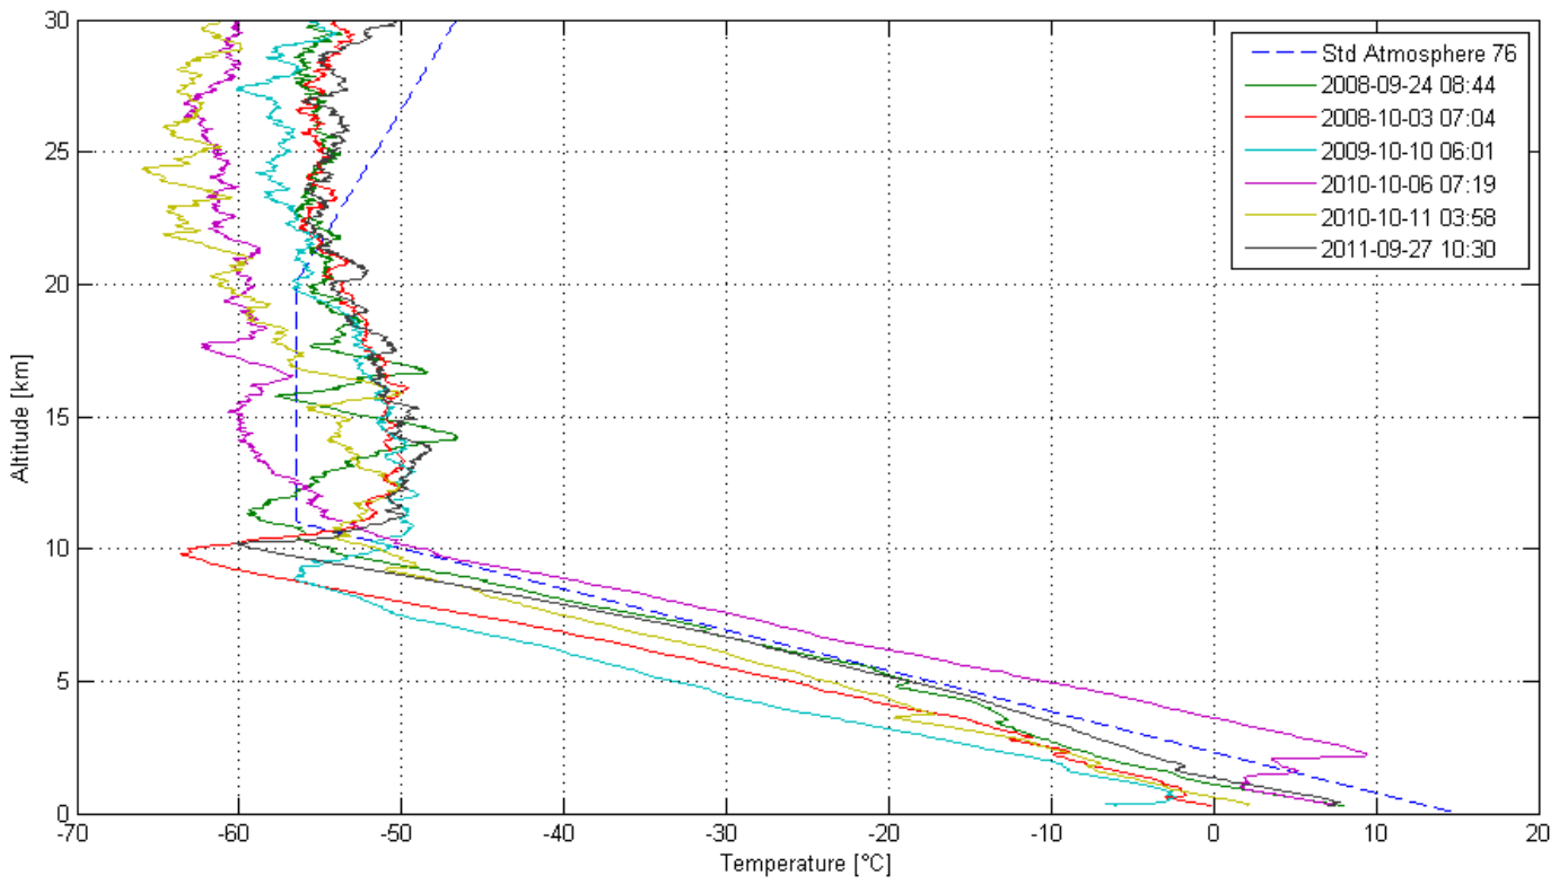
\includegraphics[scale=0.6]{4-experiment-design/img/mechanical/atmosphere.PNG}
	\caption{Temperature profile of the atmosphere. Source: REXUS/BEXUS}
	\label{fig:atmosphere}
	\end{figure}

\begin{center}
  \begin{tabular}{ | l | c | r | }
    \hline
    \textbf{Flight phase} & \textbf{Expected temperature} & \textbf{Duration} \\ \hline
    Preparation  & 15 – 25\,\textsuperscript{o}C & 4 hours \\ \hline
    Launch pad wait & -15 – 0\,\textsuperscript{o}C & 3 hours \\ \hline
    Ascent phase  & -80 – 0\,\textsuperscript{o}C & 1.5 hours \\ \hline
    Float phase (25-30km) & -70 – -50\,\textsuperscript{o}C & 1 – 5 hours \\ \hline
    Descent phase  & -80 – 0\,\textsuperscript{o}C & ~ 30 minutes \\ \hline
    Post-flight phase & -15 – 0\,\textsuperscript{o}C & 1 – 2 days \\ \hline
  \end{tabular}
\end{center}

\paragraph{Solar flux}

The extent of solar irradiance is characterised by several factors, including the sun’s height above the horizon, typically low for the polar latitudes that the balloon will be flying at, and the height in the atmosphere and atmospheric conditions, which will cause absorption and scattering of light. \\
The total solar irradiance, neglecting atmospheric effects, at the Esrange latitude of 68\textsuperscript{o} and assuming a launch date of the 15th of October is demonstrated in the following graph of direct solar radiation, with a peak of ~500\,kW/m\textsuperscript{2} at noon.\\

	\begin{figure}[h!]
    \centering
    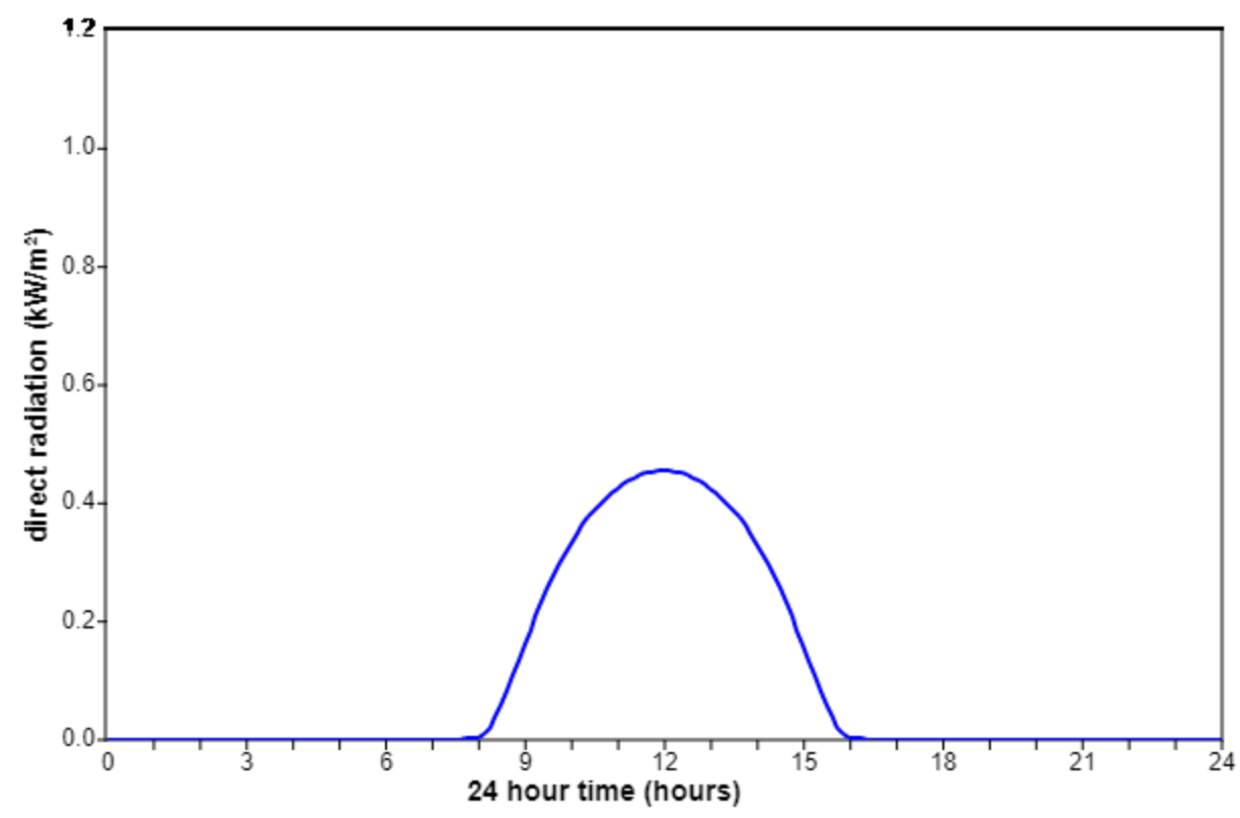
\includegraphics[scale=0.6]{4-experiment-design/img/mechanical/directradiation.png}
	\caption{Estimate of direct solar radiation at the top of the atmosphere. Source: PVeducation.org}
	\label{fig:directradiation}
	\end{figure}

The degree of attenuation of solar radiation through the atmosphere can be described using the Beer–Lambert law, which relates the transmittance of radiation to optical depth. For an atmosphere with properties that change exponentially with respect to altitude, the optical depth can be estimated to also change exponentially with respect to altitude. \\

\paragraph{Internal heat generation}
\hl{Another factor affecting the thermal environment comes from the generation of heat by the electronic components in the electronics box, from each camera, and from each motor. This heat is generated from losses of the supplied power through electrical and mechanical processes. An estimate of the power drawn by each component will be conducted.} \\

\begin{center}
  \begin{tabular}{ | l | c | }
    \hline
    \textbf{Component} & \textbf{Power drawn [W]}\\ 
    \hline
    Raspberry Pi 3B+  & 10\\
    \hline
    Gyroscope & 0.02\\ 
    \hline
    GPS  & 0.03\\ 
    \hline
    PWM controller & 0.05\\ 
    \hline 
    Encoders  & 0.04 \\ 
    \hline
    Accelerometer  & negligible \\ 
    \hline
    Temperature sensors  & negligible \\ 
    \hline
    Buck converter 3.3V  & 0.183 \\ 
    \hline
    Buck converter 5V  & 1.67 \\ 
    \hline
    Buck converter 12V  & 3.75 \\ 
    \hline
    \textbf{Total in electronics box}  & \textbf{15.78} \\ 
    \hline
    \textbf{DC motor 1}  & \textbf{1.4} \\
    \hline
    \textbf{DC motor 2}  & \textbf{1.4} \\ 
    \hline
    \textbf{DC motor 3}  & \textbf{1.4} \\
    \hline
    \textbf{Guiding camera}  & \textbf{1.5} \\
    \hline
    \textbf{Sanity camera}  & \textbf{0.825} \\ 
    \hline
    \textbf{Main camera}  & \textbf{1.5}\\ 
    \hline
  \end{tabular}
\end{center}

\hl{The DC gear motors are rated as having a maximum efficiency of 35\%. For the electronics, it will be assumed that they are 90\% efficient. By multiplying the supplied power by the efficiencies, the heat generation can be determined.} \\

\begin{center}
  \begin{tabular}{ | l | c | }
    \hline
    \textbf{Component} & \textbf{Heat generation [W]}\\ 
    \hline
    \textbf{Electronics}  & \textbf{1.58} \\ 
    \hline
    \textbf{DC motor 1}  & \textbf{0.91} \\
    \hline
    \textbf{DC motor 2}  & \textbf{0.91} \\ 
    \hline
    \textbf{DC motor 3}  & \textbf{0.91} \\
    \hline
    \textbf{Guiding camera}  & \textbf{0.15} \\
    \hline
    \textbf{Sanity camera}  & \textbf{0.08} \\ 
    \hline
    \textbf{Main camera}  & \textbf{0.15}\\ 
    \hline
  \end{tabular}
\end{center}

\hl{It is of note that in historical BEXUS projects utilising the Raspberry Pi in an insulated environment, surface temperatures of 50\textsuperscript{o}C have been recorded.} \\


\subsubsection{Temperature requirements}

\begin{center}
  \begin{tabular}{ | l | c | c |}
    \hline
    \textbf{Component} & \textbf{Component no.} & \textbf{Operating temp [\textsuperscript{o}C]} \\ 
    \hline
    Accelerometer & KXTJ3-1057CT-ND & -40 – 85 \\ 
    \hline
    ADC AD7175 & 835-3826 & -40 – 105 \\ 
    \hline
    ADC AD7997 & 697-7170 & -40 – 85 \\ 
    \hline
    Antenna & 704-3449 & -40 – 85 \\ 
    \hline
    Buck converter 3.3V & 296-40220-1-ND & -40 – 125 \\ 
    \hline
    Buck converter 5V 4A & 785-1689-1-ND & -40 – 85 \\ 
    \hline
    Buck converter 12V 1.25A & LM2695MH/NOPB-ND & -40 – 125 \\ 
    \hline
    Camera Raspberry Pi V2 & 301-34-462 & -20 – 60 \\ 
    \hline
    Camera  ZWO ASI183MM & IMX183CLK-J & -5 – 45 \\ 
    \hline
    Capacitor 1 uF & 301-19-869 & -55 – 125 \\ 
    \hline
    Capacitor 1.4 pF & 300-47-684 & -55 – 125\\ 
    \hline
    Capacitor 22 nF & 300-65-997 & -55 – 125 \\ 
    \hline
    Capacitor 44 pF (47 pF) & 300-67-381 & -55 – 125 \\ 
    \hline
    Capacitor 850 pF & 165-81-144 & -55 – 125 \\ 
    \hline
    Capacitor 0.47 uF (420 nF) & 300-87-046 & -55 – 125 \\ 
    \hline
    Capacitor 0.1 uF & 165-73-687 & -55 – 125 \\ 
    \hline
    Capacitor 1 uF & 165-61-179 & -55 – 125 \\ 
    \hline
    Capacitor 2.2 uF & 165-71-988 & -55 – 125 \\ 
    \hline
    Capacitor 3 uF (3.3 uF) & 165-71-996 & -55 – 125 \\ 
    \hline
    Capacitor 4 uF (4.7 uF) & 300-31-816 & -55 – 125 \\ 
    \hline
    Capacitor 32 uF (33 uF) & 915-5461 & -55 – 125 \\ 
    \hline
    Capacitor 10 uF & 301-12-804 & -55 – 125 \\ 
    \hline
    Capacitor 4.7 uF & 300-31-677 & -55 – 85 \\ 
    \hline
    Capacitor 0.1 uF & 300-67-806 & -55 – 125 \\ 
    \hline
    Compass & MLX90393SLW-ABA-011 & -20 – 85 \\ 
    \hline
    Crystal 16 MHz, 9 pF, 10ppm & 301-09-485 & -40 – 85 \\
    \hline
    Encoder & 102-4485-ND & -40 – 105 \\
    \hline
    Ferrite Bead 600Ohm @ 100MHz & 724-1545 & -55 – 125 \\
    \hline
    GPS & NEO-M8N & -40 – 85\\
    \hline
    Gyroscope & EVAL-ADXRS624Z-ND & -55 – 125 \\
    \hline
    Inductor 68 uH & 300-37-257 & -40 – 105 \\
    \hline
    Inductor 24 uH (22 uH) & 158-00-313 & -20 – 105 \\
    \hline
    Inductor 22 uH & 110-63-696 & -40 – 155\\
    \hline
    Igarashi DC Gearmotor & 1711491-62 & 0\textsuperscript{*} – 60 \\  
    \hline
    Microcontroller & 636-384 & -25 – 130 \\
    \hline
    Peltier cooler & PE-031-10-15-S & 0 – 74 \\
    \hline
    PWM expander & 727-5649 & -40 – 85 \\
    \hline
    Raspberry Pi Zero (no WiFi) & 1910-1104-ND & 0 – 70 \\
    \hline
    Raspberry Pi 3B+ & 137-3331 & 0 – 50 \\
    \hline
    Schottky diode & 170-09-098 & -50 – 150 \\
    \hline
    Temp sensor & 301-29-188 & -55 – 150 \\
    \hline
    Transistor NPN 15nA leak & 300-32-503 & -65 – 150 \\
    \hline
    Transistor PNP & 300-41-424 & -50 – 150 \\
    \hline
    U-regulator & 173-88-854 & -50 – 125\\
    \hline
\end{tabular}
\end{center}
\textsuperscript{*}0\textsuperscript{o}C required to prevent condensation and subsequent freezing on the motors.\\

As the ambient conditions are likely to be very cold, many of the components will need to be heated so that the electronics are able to operate.\\

\st{If the ambient conditions are assumed to be -70\,\textsuperscript{o}C, and the desired temperature for the components of 0\,\textsuperscript{o}C, heating will be needed to increase the temperature of components by up to  75\,\textsuperscript{o}C, a tolerance of 5\,\textsuperscript{o}C below the minimum operating temperature for the motors.\\} 

\hl{The Igarashi DC gearmotors will need to be maintained at between 0\textsuperscript{o}C and 60\textsuperscript{o}C. If the ambient conditions are assumed to be -70\,\textsuperscript{o}C, then the temperature of these motors will need to be raised by more than 80\,\textsuperscript{o}C, assuming a tolerance of 10\,\textsuperscript{o}C.\\

The main camera (ZWO ASI183MM) will need to be maintained at between -5\textsuperscript{o}C and 45\textsuperscript{o}C. The temperature of this component will need to increase by more than 75\,\textsuperscript{o}C. Likewise for the sanity camera. For the main camera to reduce noise there is value in keeping the optics cool while the electronics are warmed to the operating temperature. This should be taken into account in the thermal design.\\

The guiding camera (Raspberry Pi Camera v2.1) will need to be maintained at between -20\textsuperscript{o}C and 60\textsuperscript{o}C. The temperature of this component will need to increase by more than 60\,\textsuperscript{o}C.\\

For the electronics box, the temperature will need to be between 0\textsuperscript{o}C and 50\textsuperscript{o}C, for the Raspberry Pi, the most temperature sensitive component. A temperature increase of more than 80\textsuperscript{o}C is required\textsuperscript{o}C.\\}

\subsubsection{Thermal control}
\st{In order to heat the electronics to the desired temperature, Polyimide Thermofoil Heaters supplied by Minco can be used, as they are lightweight, and commonly used to protect electronics from cold at high altitudes. A heater will be supplied for each of the three motors, for the camera, and for the electronics box. The heaters can be used to generate temperatures of up to 200\,\textsuperscript{o}C. Temperature sensors will be included next to the heaters to provide feedback that will allow the temperature to be controlled to the desired operating point.} \\


\paragraph{Insulation}

\hl{In the electronics box, a substantial amount of heat is generated by the electrical components and in particular the Raspberry Pi. This heat will convect and radiate out to the colder surroundings. By quantifying the heat generation and comparing it to the heat losses, the temperature inside the box can be determined. The heat loss can be controlled by adding an insulating layer around the box, which will resist the conduction of energy to the surface of the box. In this case, extruded polystyrene will be used as the material, due to its low conductivity and because it is less resistant to thermal expansion.} \\

\hl{An analysis of the heat loss for the electronics box maintained at 20\textsuperscript{o}C was conducted.} \\

	\begin{figure}[h!]
    \centering
    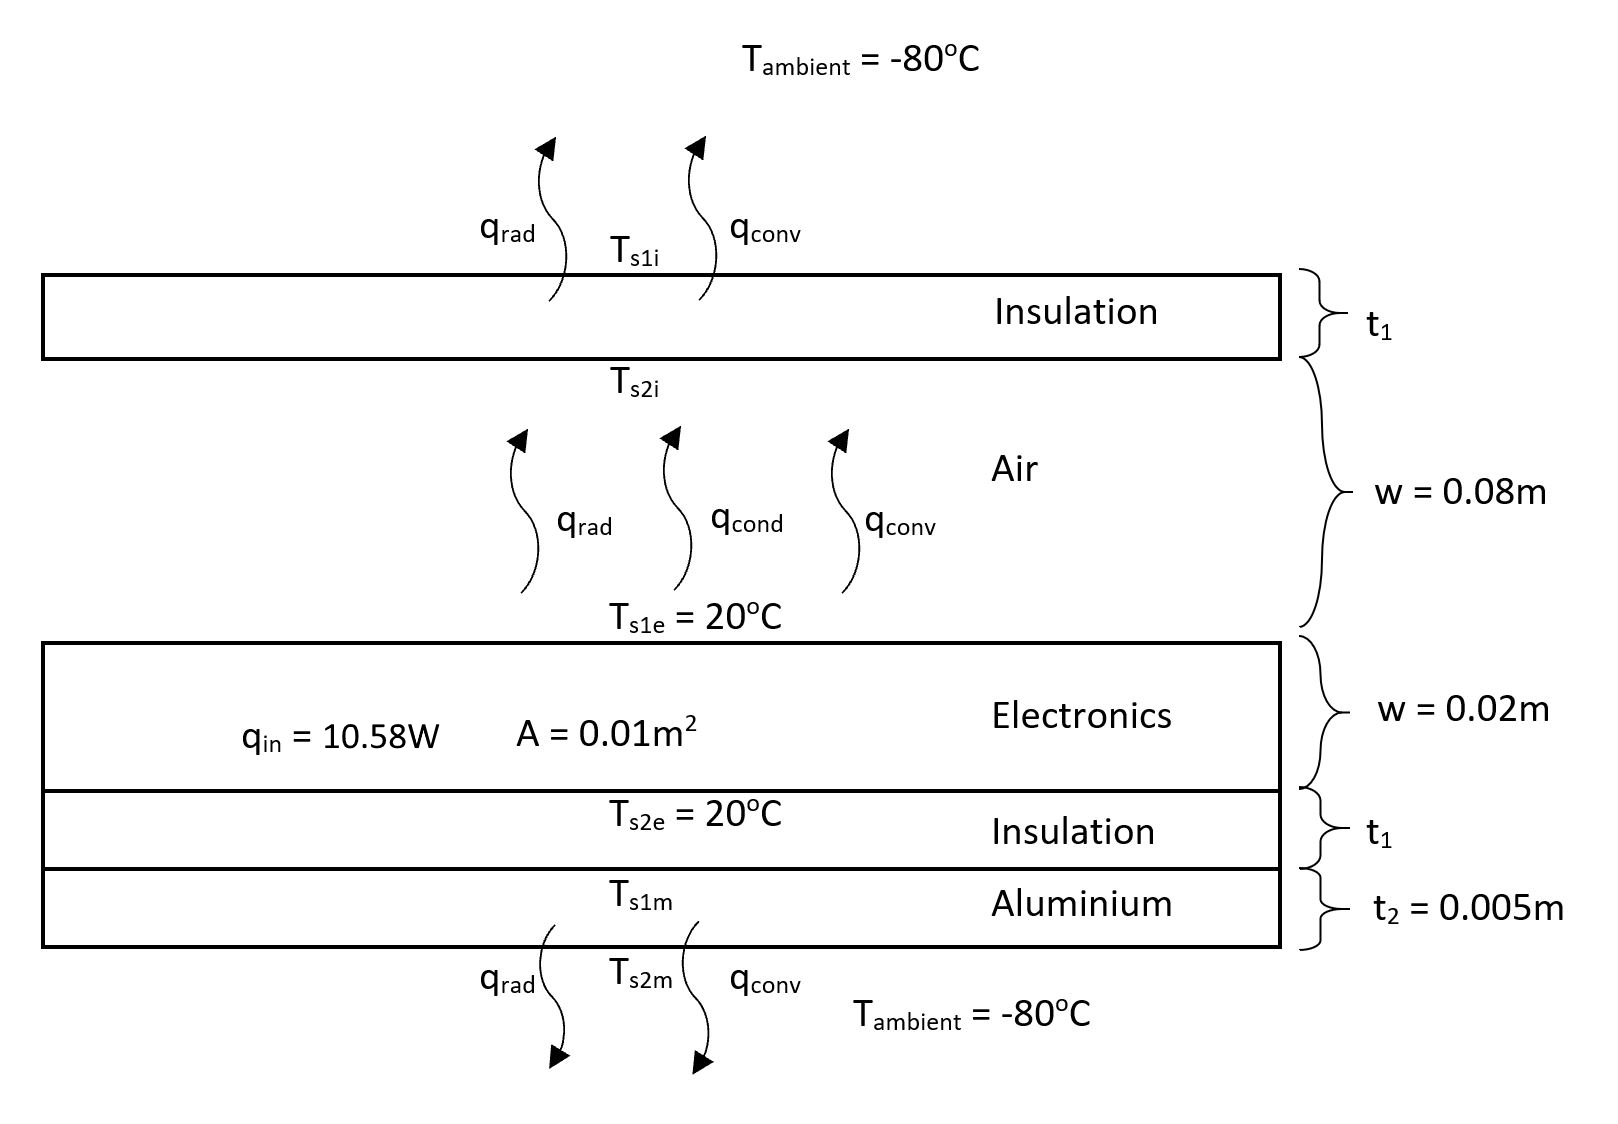
\includegraphics[scale=0.6]{4-experiment-design/img/mechanical/thermaldiagram.JPG}
	\caption{Heat transfer model of the electronics box.}
	\label{fig:thermaldiagram}
	\end{figure}

\hl{The material properties are as follows:} \\

\hl{Thermal conductivity of insulation:} $ k_{i} = 0.034 \frac{W}{m K} $ \\
\hl{Thermal conductivity of aluminium:} $ k_{m} = 205 \frac{W}{m K} $ \\
\hl{Thermal conductivity of air at 1 kPa, -80\textsuperscript{o}C:} $ k_{a} = 15\times10^{-3} \frac{W}{m K} $ \\ 
\hl{Convective heat transfer coefficient of air:} $ h_{a,c} = 3.12 \frac{W}{m^{2} K} $ \\ 
\hl{Radiative heat transfer coefficient of air:} $ h_{a,r} = 6.59 \frac{W}{m^{2} K} $ \\ 

\hl{For 1D steady state conduction through the composite wall comprised of insulation and aluminium:} \\

	\begin{figure}[h!]
    \centering
    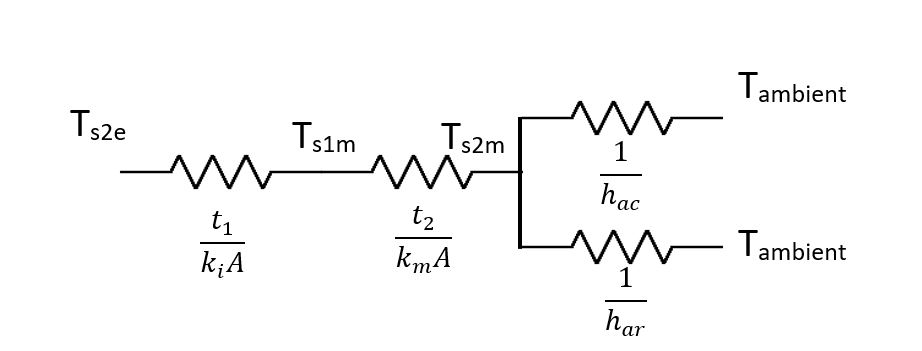
\includegraphics[scale=0.6]{4-experiment-design/img/mechanical/thermalresistance1.JPG}
	\caption{Thermal resistance for bottom of box.}
	\label{fig:thermalresistance1}
	\end{figure}

\begin{center}
 $q_{cond1} = \frac{T_{s2,e}-T_{ambient}}{R_{tot}} $\\
 
 \ 
 
 $R_{tot} = \frac{t_{1}}{k_{i}A} + \frac{t_{2}}{k_{m}A} + \frac{1}{h_{a,e}+h_{a,m}} $\\
 
 \
 \ 
 
 $q_{cond1} = \frac{293.15 - 193.15}{\frac{t_{1}}{(0.034)(0.01)} + \frac{0.005}{(205)(0.01)} + \frac{1}{3.12+6.59}} $\\
 
 \  
 \ 
 
 $q_{cond1} = \frac{100}{2940t_{1}+0.105} $\\
 
\end{center}
 

\hl{For 1D steady state conduction through the upper insulating layer:} \\

	\begin{figure}[h!]
    \centering
    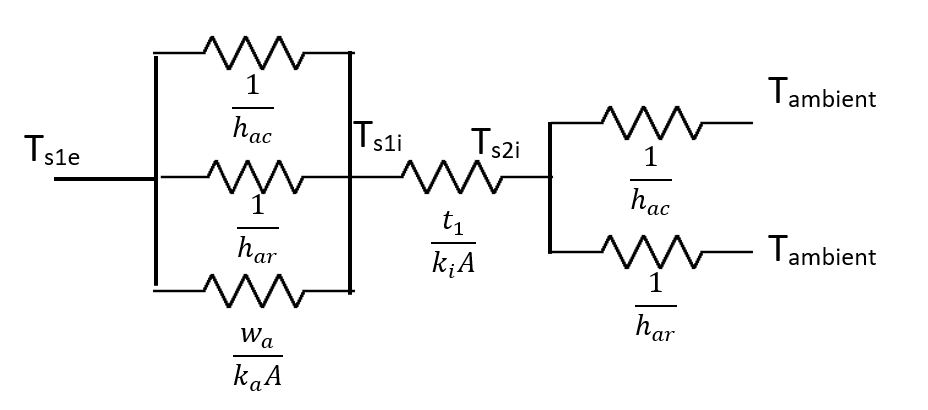
\includegraphics[scale=0.6]{4-experiment-design/img/mechanical/thermalresistance2.JPG}
	\caption{Thermal resistance for top of box.}
	\label{fig:thermalresistance2}
	\end{figure} 

\begin{center}
 $q_{cond2} = \frac{T_{s1,e}-T_{ambient}}{R_{tot}} $\\
 
 \ 
 
 $R_{tot} = \frac{1}{h_{a,e}+h_{a,m}+\frac{k_{a}A}{w_{a}}} + \frac{t_{1}}{k_{i}A} + \frac{1}{h_{a,e}+h_{a,m}}  $\\
 
 \
 \ 
 
 $q_{cond2} = \frac{293.15 - 193.15}{\frac{1}{3.12+6.59+\frac{(15\times10^{-3})(0.01)}{0.08}} + \frac{t_{1}}{(0.034)(0.01)} + \frac{1}{3.12+6.59}} $\\
 
 \  
 \ 
 
 $q_{cond2} = \frac{100}{2940t_{1}+0.206} $\\
 
\end{center}

\hl{By summing the heat lost on both sides and equating that to the heat generated, we can find the thickness of insulating material to maintain the constant temperature.} \\

\begin{center}
 $q_{loss} = \frac{100}{2940t_{1}+0.105} + \frac{100}{2940t_{1}+0.206} = 1.58 W = q_{gain} $\\
\end{center}

\hl{Solving this equation yields a thickness of 4.3 cm. It is important to note that this analysis relies on several assumptions, such as one dimensional steady state heat transfer, and that the convection mechanism on the top and bottom of the electronics box is the same. It also does not take into account heat flux from solar radiation. In reality, there will be a conductive path through the insulating material from the bottom to the top of the box, and heat will not have to pass through the very low density air in the box. This will be taken into account in a FEA analysis of the thermal properties, using the ANSYS package.} \\

\paragraph{Heating pads}

\st{The motor is 37.8\,mm long with a diameter of 33\,mm, so the 5572 heater with dimensions 12.7\,mm x 12.7\,mm and a resistance of 26.5}\,\si{\ohm} \st{is selected.}\\

\begin{center}
 $P = \frac{\SI{5}{V}\textsuperscript{2}}{\SI{26.5}{\ohm}} = \SI{0.95}{W} $\\
\end{center}

\st{The camera is 73.5\,mm long with a diameter of 78\,mm, so the 5587 heater with dimensions 31.8\,mm x 31.8\,mm and a resistance of 13.1}\,\si{\ohm} \st{is selected.}\\

\begin{center}
 $P = \frac{\SI{5}{V}\textsuperscript{2}}{\SI{13.1}{\ohm}} = \SI{0.95}{W} $\\
\end{center}

\st{The electronics box is 100\,mm x 100\,mm x 100\,mm, so the 5592 heater with dimensions 44.5\,mm x 44.5\,mm and a resistance of 26.3}\,\si{\ohm} \st{is selected.}\\

\begin{center}
 $P = \frac{\SI{5}{V}\textsuperscript{2}}{\SI{26.3}{\ohm}} = \SI{0.95}{W} $\\
 \end{center}
 
\hl{For the three motors and three cameras insulation will not be possible. For these components therefore Minco Polyimide Thermofoil heating pads will be used. These heating pads are able to increase the temperature of a target by up to 200\textsuperscript{o}C, more than enough to reach the required temperature range for the motors and cameras given the temperatures in the stratosphere.}\\

\hl{Assuming all the heat is transferred directly to the component, the power can be related to the time required to increase the target temperature by a certain amount.}

\begin{center}
 $P = \frac{mC_{p}(T_{f}-T_{i}}{t} $ \\
\end{center}

\hl{For the motors with a mass of 142\,g and made of steel with a specific heat of 0.50\,J/g/$^\circ$C, to raise the temperature by 10 degrees in 5 minutes we require 2.37 W of power. It is assumed that the camera is of similar properties.} \\

\begin{center}
 $P = \frac{(142)(0.5)(10\textsuperscript{o}C)}{5(60)} = \SI{2.37}{W} $ \\
\end{center}

\hl{This can be related to the resistance of the required heating pad.}

\begin{center}
 $P = \frac{V\textsuperscript{2}}{R} $\\

\end{center}

\hl{ By selecting the pad with resistance 52.3\,$\Omega$ and running it at 10V, it will generate 1.91W of power, and will raise the temperature by 10 degrees in 6 minutes and 11 seconds.}\\ 
 
\hl{This pad is the HK5165R52.3L12, capable of supplying 15W at 28V and has dimensions 25.4\,mm x 76.2\,mm.}\\

\hl{Given that the components are to be maintained at 20\textsuperscript{o}C, the maximum allowable watt density can be found, after which overheating and burning of the heating pad will occur. This will help to determine the application method of the pad to the heat sink.} \\

\hl{The area of the heater is 3\,inch$^2$. Dividing the power by this area yields a power density of 0.634\,W/inch$^2$. }

	\begin{figure}[h!]
    \centering
    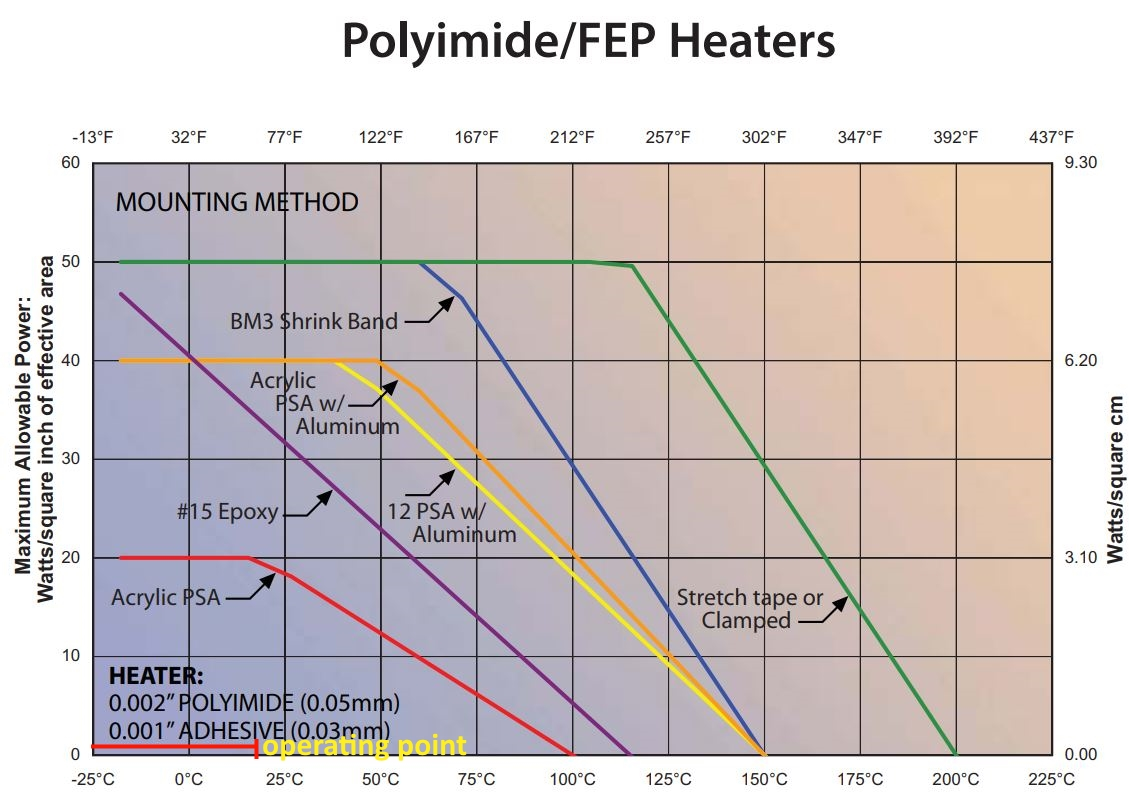
\includegraphics[scale=0.6]{4-experiment-design/img/mechanical/wattdensity.JPG}
	\caption{The maximum allowable watt density for different application methods for a given heat sink control temperature. Source: Minco heaters}
	\label{fig:thermalresistance1}
	\end{figure}

\hl{As this is low that burning of the heater is unlikely to occur, unless the temperature is not properly regulated and the heating pad warms well beyond the desired control temperature. Also, any application method is suitable with respect to this concern. The BM3 shrink band Polyaimide strip will be used as it allows heaters to be attached to cylindrical surfaces, and has a temperature minimum rating of -73\textsuperscript{o}C, lower than alternatives, making it more suitable for use in the stratosphere.}  \\

\paragraph{Thermal control}

\hl{To regulate the heater power output to ensure the required operating temperature is maintained, 6 Adafruit 165 temperature sensors will be used to provide feedback to a PID controller. These sensors can measure between -40\textsuperscript{o}C and 125\textsuperscript{o}C, with a resolution of 2\textsuperscript{o}C. Seven sensors will be used, one at the heating pad for each of the three cameras, one at the heating pad for each of the three motors, and one in the electronics box, so that recordings of the Raspberry Pi temperature can be made.} %\\

	\begin{figure}[h!]
    \centering
    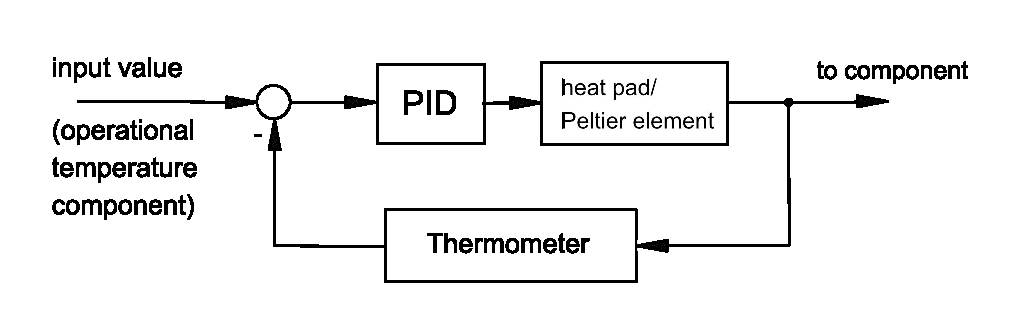
\includegraphics[scale=0.6]{4-experiment-design/img/mechanical/Thermal_control.eps}
	\caption{Schematic of the thermal control.}
	\label{fig:Thermal_control}
	\end{figure}
%\\

\hl{The motivation behind PID control as opposed to switching the heaters on and then off when they get too hot, is that the temperature will be able to converge over time to a predictable and maintained design temperature, without regular oscillations. PID control mitigates the droop of temperature below the set point that one would experience with PD control. The controller will need to be designed to ensure that the initial overshoot does not raise the temperature above the maximum operating temperature of the components, and this can be verified in testing.}    

%\\
	\begin{figure}[h!]
    \centering
    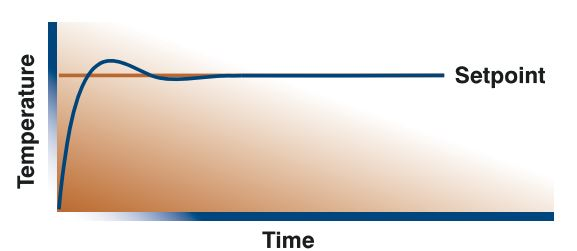
\includegraphics[scale=0.6]{4-experiment-design/img/mechanical/proportionalcontroltemp.JPG}
	\caption{PID control response over time for temperature. Source: Minco heaters}
	\label{fig:PIDcontroltemp}
	\end{figure}
%\\

